%----------------------------------------------------------------------------
\section{Introduction}\label{sect:introduction}
%----------------------------------------------------------------------------
The verifying compiler is a grand challenge in computing, perhaps most famously stated by Tony Hoare in 2003\cite{hoareGrandChallenge}, but based on research into program correctness stretching back to the 1960s\cite{hoareAxiomaticProgramming}.  Such a compiler would ideally eliminate the need for testing to reveal functional bugs by accomplishing what testing cannot: demonstrating the \emph{absence} of any bugs.  Unlike testing and informal reasoning, formal verification demonstrates that code behaves as specified under every possible valuation and along every possible path of execution.

As a powerful demonstration of the weakness of traditional testing and informal reasoning, we consider the case of binary search.  Binary search is a simple, well-understood, and widely-implemented algorithm.  Yet, Joshua Bloch of Google Research wrote a blog post\cite{blochBinarySearch} in 2006 about a subtle bug in the standard Java library's implementation of binary search---an implementation that had been in place for nine years and was based on a version of the algorithm ``proven'' correct (via informal reasoning) by Jon Bentley of Carnegie Melon University in his famous \emph{Programming Pearls}\cite{bentleyProgrammingPearls}.  Certainly, such a straightforward implementation of such a simple algorithm, backed, as it was, by a proof from a respected algorithms guru and in wide deployment for nine years would be considered by most as a \emph{mature}, \emph{well-tested} component---one suitable for use in critical deployments.  And yet it contained a subtle, latent overflow bug revealed not by a nit-picking graduate student but by a client in the wild whose code broke when the component failed to meet its specification (specifically causing an \texttt{ArrayIndexOutOfBoundsException}, which, in a C or \cplusplus context, would be a recipe for a buffer overflow attack in addition to a potential crash.)  This bug, so subtle and resilient against traditional testing and human reasoning, becomes extremely shallow under formal reasoning, where bounded, programmatic integers are well-specified in a mathematical way.

Several systems for formal verification exist, including some built on Java which may have caught this and other bugs.  These systems are traditionally built as a pipeline in which code and its associated specification are translated into an intermediate \emph{assertive code}, which is then translated into a series of \emph{verification conditions} (VCs), which express the proof obligations of the code in a purely mathematical way, before finally being sent to one or more \emph{automated provers} which attempt to dispatch the VCs.  This process is illustrated in Figure \ref{fig:pipeline}.

\begin{figure}
  \centering
    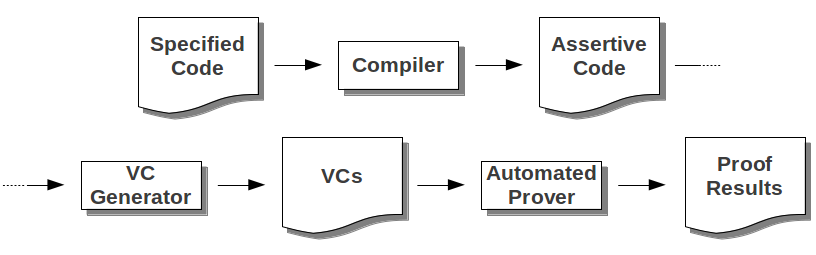
\includegraphics[width=\textwidth]{verification_pipeline}
  \caption{The Verification Pipeline\label{fig:pipeline}}
\end{figure}

Despite many successes, all existing systems require a great deal of effort, either in the form of interactive proving or carefully contrived hints to an automated prover, in order to verify even simple programs.  This is counter-intuitive since most programs contain straight-forward logic that the programmer feels assured of without calling upon complex mathematical reasoning.  The problem is compounded by a lack of integration between between modern, modular programming languages and expressive, flexible mathematics that prevents the design of reusable components, which could amortize this intense verification effort over time.  We hypothesize that a well-integrated, flexible and extensible mathematical and specification subsystem would permit specifications that more closely reflect the programer's intuition and the usual patterns of reuse, resulting both in more straightforward proofs and more generic, longer-lived components.  This proposal seeks to develop such a system and test this hypothesis.

%----------------------------------------------------------------------------
\subsection{Existing Systems: Practical vs. Pure}
%----------------------------------------------------------------------------
Existing verification systems largely fall into two categories: those with a focus on practical, automated verification and those with a focus on pure mathematics.  Examples of the former include Jahob\cite{kuncakJahobOverview}, based on Java; Spec\#\cite{specsharp}, based on C\#; and ACL2\cite{kaufmannACL2}, based on Lisp.  Examples of the latter include Coq\cite{coq}, based on the Calculus of Inductive Constructions; and Isabelle\cite{nipkowIsabelle}, based on a higher-order, intuitionistic logic.  Practical systems often take advantage of a limited, hardcoded mathematical universe that corresponds closely to or is conflated entirely with programming constructs.  Pure systems permit an extensible, flexible mathematical framework with clear separation of programming concepts from mathematics.  Because of their narrower focus, the former often permit easier mechanical verification than the latter\footnote{Some systems even permit efficient decidable verification algorithms for certain domains or properties.  See, e.g., information on SplitDecision in \cite{Sit11}.}, which tend to emphasize interactive user-guided verification.

%----------------------------------------------------------------------------
\subsubsection{Example Practical System: Jahob\label{sec:exPractical}}
%----------------------------------------------------------------------------
Let's consider a version of Java's \texttt{ArrayList} verified in Jahob\footnote{Jahob does not yet work with Java generics and so the version of ArrayList verified is the pre-Java-1.5 version that operates on \texttt{Object}s.}.  Jahob combines code written in a subset of Java with specifications written in Isabelle.  Listing \ref{lst:alcontains} shows the \texttt{contains()} operation of an ArrayList.

\lstinputlisting[language=Java,caption={ArrayList.contains()\label{lst:alcontains}}]{ArrayList1.java}

The list is modeled as a set of $(index, element)$ pairs.  Assertions are provided inside Java comments (meaning that Jahob-specified Java programs remain compilable using a standard Java compiler) that begin with a colon.  Note that mathematical assertions are set off in quotes, a syntax inherited from Isabelle.  \texttt{init} is a predicate defined elsewhere in the class.  Jahob encourages the inclusion of inline ``hints'' targeted at the backend provers\cite{zeeIntegratedProofLanguage} (of which it supports many) and we see several of those here interspersed in the Java code.

Utilizing a suite of provers, the Jahob system is able to dispatch the resultant VCs and yield a fully-verified \texttt{ArrayList} implementation suitable for generic use---an impressive feat.  In fact, in a recent result, the Jahob team verified a handful of different linked data structures\cite{zee:annotations}.  A number of design decisions support this ability.  First, Jahob has a flexible set of syntactic tools for specification, including pre- and post- conditions, auxiliary variables\cite{kingVerifier}, and conceptual definitions that permit an intuitive specification.  Second, while Jahob supports higher-order specifications, where possible it uses a standard first-order logical representation that can be translated into the input format of multiple back-end proving systems including CVC3\cite{barretCVC3} and Z3\cite{deMouraZ3}.  Those specifications that cannot be translated down to a first-order representation can still be sent to Isabelle for interactive proving.  By using multiple prover backends, Jahob can take advantage of multiple proving paradigms including interactive, algebraic, boolean satisfiability (SAT) solvers, and efficient decision procedures.  Third, as already stated, Jahob permits in-line mathematical assertions that allow the programmer to guide backend provers by stating useful intermediate results.

However, despite this success, a number of the realities of this system (and others like it) are counter-intuitive and seem geared toward short-term verification of small Java programs rather than long-term, scalable verification of complex, modular applications.

\paragraph{Complex Proof Obligations for Simple Methods.\label{sec:jahobComplexVCs}}
When using the Jahob system, VCs that result from even simple programs are often extremely complex. Jahob's intermediate VC syntax is not intended to be human readable, so we do not reproduce any VCs here, but we can get a feel for their complexity via sheer volume: the three-line boolean method \texttt{contains()} generates VCs that span over 150 lines\footnote{When formatted to standard 80-character lines.}.  

A number of factors contribute to this VC complexity.  First, Jahob is built on top of an existing programming language that includes many features that are not amenable to verification, including null pointers and uncontrolled aliasing, both of which complicate reasoning\cite{weideVerificationReferences}.  These complexities must be accounted for in its VCs.  Second, Jahob's inline assertions must themselves be verified to preserve soundness.  The intent of these assertions is that they simplify the proving process by proving intermediate steps, creating additional (presumably easier) VCs that in turn lower the difficulty of the original proof obligations.  Still, why intermediate results should be required for a simple \texttt{contains()} method is unclear.  Third, while perhaps subjective, the system encourages the use of awkward mathematical models for components.  In the list example, the choice of a set for mathematical model requires additional invariants to establish that, for example, no index in the list appears twice with different elements.  Presumably a set was chosen because it was the closest mathematical object that already had a well-developed Isabelle theory, but in an ideal world such a system would provide a first-class, integrated mechanism for extending the mathematical universe so that a more directly analogous mathematical object could be used---perhaps a function mapping or a finite sequence abstraction.

\paragraph{Lack of Support for Modular Design.\label{sec:jahobNoModularity}}
Jahob stands nearly alone amongst the practical systems for supporting higher-order mathematics.  However, practical issues with the integration of Isabelle into Java hamstring the usefulness of this feature.  Among the Java features not supported by Jahob are Java generics and dynamic dispatch.  These unsupported features preclude many important patterns of reuse that the mathematics of Isabelle are otherwise ready to support.  Components cannot be parameterized from the outside with definitions (this is not supported directly and programmatic work-arounds like the Strategy and the Template design patterns rely on dynamic dispatch.)  Data structures cannot make parameterizable guarantees about the properties of contained elements (which would require Java generics.)  Indeed, the majority of the polymorphism pillar of object-orientation is precluded, seriously reducing the reusability of components and thus the amortization of verification effort over time.

A particularly illustrative example of this lack of modularity appears in a \texttt{Map} data structure verified by the Jahob team in \cite{zee:annotations}.  The trouble of aliased keys is dealt with by specifying that \emph{all objects} are immutable with respect to the built in Java \texttt{hashcode()} method---a restriction that does not appear in the original \texttt{Object} contract and further implies that all objects are immutable with respect to \texttt{equals()}.  The correctness of the \texttt{Map} implementation requires changes to external components, rather than being part of its self-contained specification.  We discuss this problem in more detail in \cite{bronishMap}.

\vspace{1.5em}With lengthy, complex VCs, syntax for guiding back-end provers, and a system that encourages a trade-off of mathematical flexibility for prover diversity, the Jahob design seems to assume that the onus of verification is on the provers.  It shifts the complexity of verification to the part of the pipeline highlighted in Figure \ref{fig:prover}.  However, as the strength of automated provers is the current bottleneck of verification, this requires a great many sacrifices to the limitations of this bleeding-edge part of the verification toolchain.

\begin{figure}
  \centering
    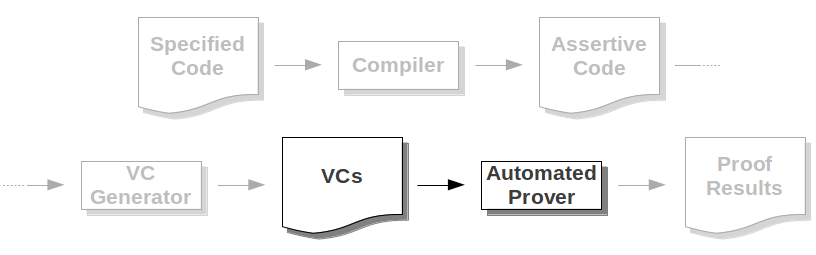
\includegraphics[width=\textwidth]{proverpart}
  \caption{Shifting the Burden to the Prover\label{fig:prover}}
\end{figure}

%----------------------------------------------------------------------------
\subsubsection{Example Pure System: Coq\label{sec:exPure}}
%----------------------------------------------------------------------------
Let's consider a recursive implementation of the integer division operator, specified and implemented in Coq.  Despite the fact that Coq is a mathematical system, unable to execute code, we could use its ability to ``extract'' a program into various target languages\footnote{At time of writing: OCaml, Haskell, and Scheme.} for execution.  Coq separates specification from implementation; in Listing \ref{lst:divpred} we see a pair of predicates for specifying integer division.

\lstinputlisting[language=Coq,caption={Division Predicates\label{lst:divpred}}]{DivPred.coq}

The \texttt{divPre} predicate represents the precondition on division---that the second argument is not 0.  The \texttt{divRel} predicate specifies the relational behavior of division---that the result will consist of two natural numbers, \texttt{q} and \texttt{r}, such that \texttt{q * d + r = n} and \texttt{r < d}, i.e., \texttt{q} is the quotient and \texttt{r} the remainder.

We then implement division recursively as shown in Listing \ref{lst:divimpl}.

\lstinputlisting[language=Coq,caption={Division Implementation\label{lst:divimpl}}]{DivImpl.coq}

Coq's \texttt{Function} keyword introduces a recursive function with an appropriate implicit fixpoint.  The \texttt{measure} keyword provides a progress metric---namely, that \texttt{fst} is decreasing.  Note that, despite the fact that an input matching \texttt{(\_,0)} is disallowed by the precondition, Coq does not permit non-total functions, so we provide a nonsense return value for this case.  The \texttt{le\_lt\_dec} is simply a less-than-or-equal-to predicate on natural numbers. Defining this function immediately raises a termination proof obligation, which one of Coq's built-in proof scripts can dispatch automatically.

To demonstrate the correctness of the implementation, we can assert the theorem given in Listing \ref{lst:divtheorem}.  That is, that for all inputs, if the inputs meet the precondition, then the behavioral relation holds between the inputs and the result of applying \texttt{div}.

\lstinputlisting[language=Coq,caption={Division Functional Correctness Theorem\label{lst:divtheorem}}]{DivTheorem.coq}

Proving this theorem is more complicated than the termination proof and none of Coq's built-in tactics can dispatch it automatically.  Instead we enter interactive mode and prove it live with the sequence of tactics given in Listing \ref{lst:divproof}.

\lstinputlisting[language=Coq,caption={Division Functional Correctness Proof\label{lst:divproof}}]{DivProof.coq}

A high-level sketch of this proof is that it applies induction by cases, proving that each of the \texttt{match} branches and each of the \texttt{if} branches maintains the correctness of the implementation.  Definitions are repeatedly expanded to take advantage of their hypotheses.  Obviously, however, this syntax is far from readable without being intimately familiar with Coq and certainly looks nothing like a mathematical proof as it might be conceived by a mathematician.

Systems like this have been used to excellent effect verifying complex programs.  Coq has been used to verify a C compiler\cite{leroyVerifiedcompiler}, while Isabelle has been used to verify an operating system kernel\cite {kleinVerifiedOS}.

This success is due to a number of factors.  Unlike in the practical programming systems, Coq and other pure systems provide a rich, extensible mathematical universe permitting higher-order logic and user-created mathematical theories.  This enables a hierarchy of abstraction similar to the development of object oriented code in which complex mathematical objects are repeatedly decomposed into smaller and smaller mathematical objects and an ``interface'' of theorems is provided for working with the high level objects.  In addition, Coq's programming model is functional, eschewing a number of complexities pervasive in industrial languages---pointers, aliasing, and referential opacity to name a few.  Automated proof systems are used to jump small steps, but interactive mechanisms are provided for splitting complex proof obligations into multiple smaller tasks.  It's as though the human user becomes part of the assertive code and VC generation step, pointing out useful decompositions of existing proof obligations until they become small enough that the automated prover can take it from there.  In a sense, such a system shifts the onus of the verification process to the part highlighted in Figure \ref{fig:assertivecode}.

\begin{figure}
  \centering
    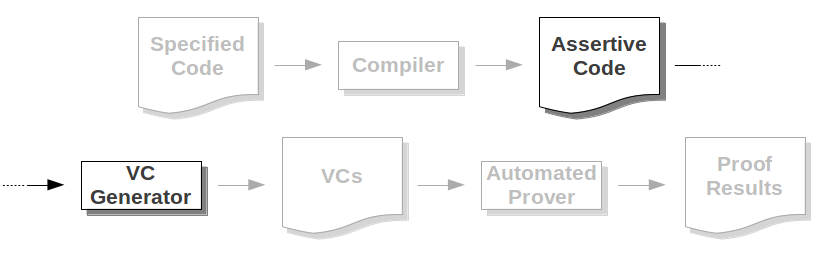
\includegraphics[width=\textwidth]{vcpart}
  \caption{Shifting the Burden to the VC Generator\label{fig:assertivecode}}
\end{figure}

Unfortunately, given the value of a highly-trained mathematical and programming professional's time, a user-guided strategy is likely cost-prohibitive if all but the smallest proof obligations must be discharged by hand.  A number of factors contribute to the difficulty of these proof obligations.

One is that, in order to exploit the flexibility of the mathematical system, the automated prover must be more general, unable to take advantage of the numerous domain-specific tricks that cutting-edge narrowly-applicable theorem provers exploit.  Another is that the divide between the mathematical world of Coq and the programming world of an industrial language is large.  We see an example of this in the division example, where time and effort must be expended proving that the behavioral relation is total (even though the method it specifies is not!) and that an irrelevant program branch maintains invariants.

Compounding this problem, pure systems have no awareness of the underlying programmatic structure they are being applied to and thus inherently view verification as operating on procedural rather than object-oriented code.  Modular mathematics are therefore not applied to modular code and the result is that, impressive as a verified compiler is, the next complex component must be verified from scratch as it is unlikely that any component from the compiler will be generic enough to be reusable.

%----------------------------------------------------------------------------
\subsection{Best of Both Worlds?}
%----------------------------------------------------------------------------
At the core of this research is the question of whether or not a system that combines the best parts of practical systems and the best parts of pure systems might permit specifications that are more amenable to automatic verification.  A programming system that eschews certain complexities of industrial languages and avails itself of a tightly-integrated, flexible and extensible mathematical system designed to work with it could be used to create modular components based on modular mathematics.  We hypothesize that in such a system, a focus on modularly verified components would yield less complex proof obligations while at the same time encouraging the creation of reusable components that amortize the verification effort invested in them over time.  Such a system would place the onus of the verification on the design of modular specifications supported by a flexible compiler, i.e., that part of the pipeline highlighted in Figure \ref{fig:specification}.  Highly trained programmers and mathematicians are still required, but the fruits of their labors will be generic and reusable, unlike proofs of correctness.

\begin{figure}
  \centering
    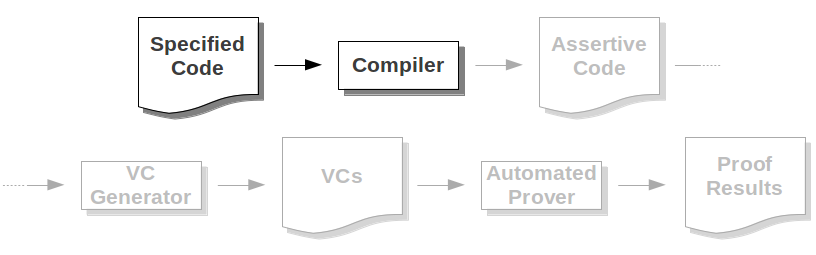
\includegraphics[width=\textwidth]{specpart}
  \caption{Shifting the Burden to Specification\label{fig:specification}}
\end{figure}

Developments such as these would also benefit existing systems of all types.  Increased understanding of the importance and techniques of modular reasoning can be applied to systems like Jahob to increase the provability of large components via better-engineered subcomponents.  A richer understanding of the importance of levels of mathematical abstraction to long-term verification goals would assist those working in pure system like Coq in making better up-front choices to pay long-term dividends.

%----------------------------------------------------------------------------
\subsection{Problem Statement}
%----------------------------------------------------------------------------
This proposal seeks to determine if the mechanical verifiability of software components can be improved by better-engineered mathematics and specifications and, if so, explore which techniques might best support these goals.  In the process it will address the following open problems in the area of formal methods:

\begin{itemize}
\item Design of an extensible, flexible mathematical framework and a well-integrated associated specification framework, supporting verifiability by allowing specifications based on the \emph{best} mathematical model, rather than simply the most convenient, and supporting scalability through mathematical reuse.
\item Architecture of and experimentation with a minimalist rewrite prover to support reasoning in the above framework and determine those prover capabilities practically necessary to mechanically verify well-engineered, modular components.
\item Creation of a diverse library of components of the sort found in standard programming libraries, specified and modeled using a broad set of techniques to enable experimentation on mathematical and specification best-practices for practical verification.
\end{itemize}

%----------------------------------------------------------------------------
\subsection{Research Approach}
%----------------------------------------------------------------------------
Building on previous work on specification language design, VC generation, and automated prover development, this research seeks to augment the existing RESOLVE\cite{Sit11} system with a flexible mathematical subsystem and modular specification subsystem in order to experiment with the specification and mathematics best-practices in support of modularity.

Unlike practical systems, where bringing modular mathematics to bear in support of modular programming is difficult at best and where special-case constructs like references cause complex reasoning even in situations where they ought not be relevant, the mathematical system proposed here will be tightly integrated and based on an extensible Morse-Kelley Set Theory, extended to include higher-order definitions, and will permit specification of programmatic constructs (e.g., references) only as modeled in that pure mathematical system.

Unlike pure systems, where the specification system that bridges between mathematics and programming is ad-hoc and not designed to take advantage of the structure of a program, the specification system proposed here will cooperate with the mathematical system by design, thus permitting it to take advantage of the same modularity and genericity used in a well-designed component.

Armed with such a system, we will test its flexibility by designing, specifying, and implementing a library of programming components ranging from simple stacks to more complicated tree structures, along with the algorithms for manipulating these structures.  These structures and algorithms will be modeled and specified using a variety of techniques in order to gain insight into how these techniques impact verifiability and scalability.  We will analyze resulting VCs to determine which prover capabilities are strictly necessary, designing and building a minimalist rewrite-based prover based on a plug-in architecture to support only those capabilites necessary for practical VCs.

The evaluation of the system as a whole will include classification of VCs by the minimalist prover based on a number of proof metrics including number of required theorems, number of required proof steps, and proof time; as well as subjective, qualitative metrics derived from field tests with programming and mathematics students and professionals.

%----------------------------------------------------------------------------
\subsubsection{Contributions\label{sec:contributions}}
%----------------------------------------------------------------------------
Such a system would address several open problems in the area of formal methods, both practical and theoretical:

First, a flexible, extensible, and intuitive mathematical subsystem would significantly improve on a key component of the verification tool chain.  The day when an AI can infer the intent of a program and verify it without rigorous specification and significant mathematical development is extremely distant.  Until that time, formal verification will be a joint effort between highly trained programmers and mathematicians.  While improvements are being made\cite{wenzelIsar}, the current generation of specification systems (both practical and pure) largely use ad-hoc mathematical syntax and esoteric mathematical foundations that programmers may find convenient but mathematicians find confusing and unweildy.  Beyond simply engendering collaboration between programmers and mathematicians, such a math-centered language design will encourage the full body of modern mathematical developments to be used directly.  Additionally, since it is not grounded in any programming constructs, it will not be tied to any particular language and may itself be used as a component outside of RESOLVE.

Second, a well-integrated and flexible specification and mathematical system would open up the development of verified components to modular, reusable techniques by providing first-class syntax and flexible mathematical semantics for mapping such programmatic ideas into the mathematical realm.  As an example, the lack of useful higher-order logic in practical systems prevents components from being designed to take mathematical assertions or abstract operations as parameters, severely limiting one dimension of reuse: genericity\cite{bronishMap}.  Our hypothesis is that a well designed, modular system should better exploit programmer intuition and allow for more straightforward proof obligations, permitting slower, but more expressive, automated provers to be used.  The development of such techniques would be a boon to existing systems, as well.  For example, as part of our research so far, we have explored the concept of quantifier elimination and techniques that can be used to specify and verify in their absence.  In a recent paper from the Jahob team, we find a quote highlighting the need for such research, here in the context of an attempt to verify an implementation of a Java \texttt{ArrayList}: ``Unfortunately, the provers are unable to automatically prove the post-condition of remove.  What makes the problem...difficult is that the assumptions contain universally quantified formulas while the post-condition contains an existentially quantified formula.''  Our research on engineering mathematics addresses this and other issues and may be helpful in elliminating such complications.

Thirdly, such a system will permit the above hypothesis to be tested and demonstrated in a rigorous, mechanical environment.  The current state of the art in verification suggests that verification is hard because programs are complicated.  We believe that well-engineered programs are not complicated and that, by extension, if augmented with well-engineered specifications, the resulting proof obligations should not be difficult.  Thus, a system designed to support well-designed programs is more important to successful verification than one designed to support the limitations of a state-of-the-art prover.  What such a design entails and what it means to be a ``well-engineered specification'' are open questions addressed by this research.

%----------------------------------------------------------------------------
\subsection{Thesis Statement}
%----------------------------------------------------------------------------
In a verification system, an extensible, flexible mathematics and specification subsystem enables better-engineered component specifications and thus more straightforward proof obligations that are more easily dispatched by even minimalistic automated theorem provers.

%----------------------------------------------------------------------------
\subsection{Proposal Organization}
%----------------------------------------------------------------------------
The remainder of this proposal is organized as follows: Section~\ref{sec:background} gives an overview of the state-of-the-art in each of the problem areas, with information on work related to this research, Section~\ref{sec:resolveBackground} provides background on the RESOLVE verification system that is the platform for this research, Section~\ref{sec:research} presents the proposed research including work already completed, Section~\ref{sec:evaluation} explains the criteria against which the work will be evaluated, and Section~\ref{sec:conclusion} will offer some concluding thoughts.
